Segundo resolução da Anvisa, toda água mineral no país que possua como objetivo ser comercializada deve ser adicionada
de sais minerais. Visando seguir esta especificação e visando não provocar um impacto na saúde dos habitantes de Acarí,
optou-se por adicionar sais minerais básicos à água retirada da umidade do ar, já que a falta de sais minerais na água 
dos habitantes pode levar a doenças para os mesmos, tais como diarreia e desidratação.

Uma das propriedades mais importantes da água é o fato de ser uma substância polar, capaz de associar-se a outras substâncias
polares ou iônicas para formar soluções aquosas. O processo de solubilização para a planta de abastecimento de água por meio 
da umidade do ar pode ser realizado por um simples processo de mistura entre os sais contidos em um reservatório e a água
provinda da turbina. Tendo em vista a deficiência desses sais na água captada, é necessária a implementação de um sistema
que adicione os sais minerais em quantidades adequadas \cite{christine08}.

\subsubsection{Quantidade e especificações dos sais minerais adicionados}

  Segundo a Anvisa, a água adicionada de sais  deve ser possuir pelo menos 30ml de um dos seguintes sais, de grau alimentício:
  bicarbonato de cálcio, bicarbonato de magnésio, bicarbonato de potássio, bicarbonato de sódio, carbonato de cálcio, carbonato
  de magnésio, carbonato de potássio, carbonato de sódio, cloreto de cálcio, cloreto de magnésio, cloreto de potássio, cloreto
  de sódio, sulfato de cálcio, sulfato de magnésio, sulfato de potássio, sulfato de sódio, citrato de cálcio, citrato de magnésio,
  citrato de potássio e citrato de sódio.
  
  \begin{table}[h]
    \centering
    \begin{tabular}{|c|c|}
    
    \hline
    Substância & Quantidade(mg)\\
    \hline                               
    Cálcio & 25\\
    \hline                               
    Magnésio & 6,5\\
    \hline                               
    Potássio & 50\\
    \hline                               
    Sódio & 60\\
    \hline
    \end{tabular}
    \caption{Quantidades limites de sais minerais para cada 100 mililitros de água \cite{anvisa05}.}
  \end{table}

\subsubsection{Filtro adicionador de sais minerais}

  O sistema adicionador de sais selecionado para o projeto foi escolhido por ser simples e eficaz para o contexto do mesmo. 
  O filtro adicionador de sais escolhido é utilizado por algumas empresas espalhadas pelo mundo, estes filtros são encontrados 
  tanto em pequeno quanto em grande porte. O sistema contará com um filtro adicionador de quatro sais minerais: sódio, potássio,
  cálcio e magnésio, além de um simples sistema eletrônico para o controle da quantidade de sais minerais na água. 
  
  Sabe-se que a planta de abastecimento de água através da umidade do ar possuirá uma produção de aproximadamente 5 mil litros
  de água por dia. Desta forma, um reservatório com capacidade de 6 mil litros já estava definido com o objetivo de armazenar 
  a água produzida pela turbina. Será adicionado outro reservatório com capacidade de 6 mil litros para armazenar a água já 
  adicionada de sais.
  
  \begin{figure}[!htbp]
    \centering
    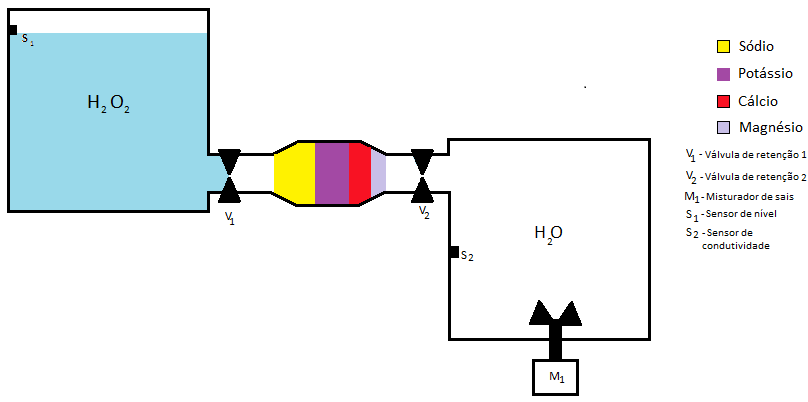
\includegraphics[scale=0.6]{editaveis/figuras/sistema_adicionador_sais}
    \caption[Esquemático do sistema adicionador de sais]{Esquemático do sistema adicionador de sais.}
    \label{sistema_adicionador_sais}
  \end{figure}
  \FloatBarrier
  
\subsubsection{Sistema de controle}

  Será utilizado um simples sistema de controle \textit{on / off} para realizar o controle das válvulas de retenção com a finalidade de 
  garantir uma concentração de sais minerais adequada para o consumo humano. 
  
  Serão utilizados dois valores de referência para o controle do sistema: um valor inferior, que representará uma quantidade mínima 
  de concentração de sais que será aferida pelo sensor de condutividade presente no reservatório dois e um valor superior, que 
  representará a quantidade máxima de concentração de sais que também será aferida pelo mesmo sensor de condutividade.
  
  Quando o valor mínimo de concentração de sais na água do reservatório dois for ultrapassado, o micro controlador do sistema
  enviará um sinal para que a válvula $V_1$ se abra completamente e outro sinal para que a válvula $V_2$ possua uma abertura mínima. Este 
  controle fará com que a água no primeiro reservatório seja contida por mais tempo no filtro de adição de sais e assim possua uma
  maior concentração de sais. 
  
  Desta forma, quando a água provinda do filtro for misturada à água do segundo reservatório, a concentração de sais deste
  reservatório aumentará. Este processo ocorrerá até o momento em que o sensor de condutividade envie um sinal para o micro 
  controlador avisando que o nível de concentração de sais do segundo reservatório chegou ao seu limite máximo. O esquemático 
  do processo pode ser visto na figura \ref{sistema_adicionador_sais}.
  
  Por outro lado, quando o valor máximo de concentração de sais na água do reservatório dois for ultrapassado, o micro controlador
  do sistema enviará um sinal para que a válvula $V_1$ e a válvula $V_2$ se abram completamente. Este controle fará com que a água no primeiro
  reservatório seja contida por menos tempo no filtro de adição de sais e assim possua uma menor concentração de sais.
  
  Desta forma, quando a água provinda do filtro for misturada à água do segundo reservatório, a concentração de sais deste
  reservatório terá a tendência de diminuir. Este processo ocorrerá até o momento em que o sensor de condutividade envie um sinal
  para o micro controlador avisando que o nível de concentração de sais do segundo reservatório chegou ao seu limite mínimo. 
  O esquemático do processo pode ser visto na figura \ref{sistema_adicionador_sais}.
  
  Os valores máximos de concentração de sais verificado pelo sensor de condutividade baseado nos valores máximos definidos pela 
  Anvisa e citados anteriormente neste documento. Os valores mínimos não serão abordados neste documento, pois precisa-se de um 
  estudo detalhado para definir a quantidade de sais necessária para o consumo humano.
  
  $M_1$ representa o motor que realizará a mistura dos sais à água provinda do primeiro reservatório de maneira mais uniforme.